% !TeX root = tcolorbox.tex
% include file of tcolorbox.tex (manual of the LaTeX package tcolorbox)
\clearpage
\section{\mylib{vignette} 程序库}\label{sec:vignette}%
\tcbset{external/prefix=external/vignette_}%
该程序库通过宏包选项或在导言区中用以下方式加载：
\begin{dispListing}
\tcbuselibrary{vignette}
\end{dispListing}
这还会加载 \mylib{skins} 程序库（参见 \zvref{sec:skins}），
以及 \tikzname\ 的 |fadings| 程序库 \cite{tantau:tikz_and_pgf}。


\subsection{装饰角绘制}\label{subsec:vignettedrawing}

\begin{docCommand}[doc new=2016-04-22]{tcbvignette}{\marg{options}}
  此处的\emph{装饰角}是一个由四部分组成的矩形边框。
  它由若干 \tikzname\ 路径构成，因此只能在 |tikzpicture| 环境内部
  或 \refEnv{tcolorbox} 选项内部使用。

  \meta{options} 控制装饰角的位置、尺寸和样式设置。
  这些选项共用键路径 |/tcb/vig/|，下文逐一说明。

  下面几个示例演示不借助 \refEnv{tcolorbox}、直接使用
  \refCom{tcbvignette} 的情况。

\begin{dispExample*}{sbs,righthand width=3cm,center lower}
\begin{tikzpicture}
  \tcbvignette{}
\end{tikzpicture}
\end{dispExample*}

\begin{dispExample*}{sbs,righthand width=3cm,center lower}
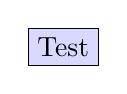
\begin{tikzpicture}
  \node[draw,fill=blue!15!white] (A) {Test};
  \tcbvignette{outside node=A,raised color=blue}
\end{tikzpicture}
\end{dispExample*}

\begin{dispExample*}{sbs,righthand width=3cm,center lower}
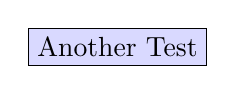
\begin{tikzpicture}
  \node[draw,fill=blue!15!white] (A) {Another Test};
  \tcbvignette{size=3mm,outside node=A,
    north style=red,east style=yellow,
    south style=blue,west style=green}
\end{tikzpicture}
\end{dispExample*}

\begin{dispExample*}{sbs,righthand width=3cm,center lower}
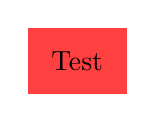
\begin{tikzpicture}
  \node[inner sep=3mm,fill=red!75] (A) {Test};
  \tcbvignette{over node=A,fade in}
\end{tikzpicture}
\end{dispExample*}

\refCom{tcbvignette} 也可直接用于 \refEnv{tcolorbox} 的相应选项键中。
注意，像 \refKey{/tcb/underlay} 这样的选项需要
\refKey{/tcb/enhanced} 或类似设置。

\begin{dispExample*}{sbs,righthand width=3cm,center lower}
\begin{tcolorbox}[enhanced,size=small,sharp corners,
  colback=green!10,colframe=green!50!black,
  boxrule=1mm,titlerule=0mm,
  title=My title,center title,fonttitle=\bfseries,
  underlay={\tcbvignette{size=1mm,inside node=frame,
      raised color=green!50!black}}]
    This is a tcolorbox.
\end{tcolorbox}
\end{dispExample*}

通常，可使用 \refKey{/tcb/underlay vignette} 之类便捷快捷方式，
为 \refEnv{tcolorbox} 添加\emph{装饰角}。此时 \refCom{tcbvignette} 在内部被调用。

\begin{dispExample*}{sbs,righthand width=3cm,center lower}
\begin{tcolorbox}[enhanced,size=small,sharp corners,
  colback=green!10,colframe=green!50!black,
  boxrule=1mm,titlerule=0mm,
  title=My title,center title,fonttitle=\bfseries,
  underlay vignette]
    This is a tcolorbox.
\end{tcolorbox}
\end{dispExample*}

\end{docCommand}



\subsection{通用几何设置}\label{subsec:vignettegeometry}


\begin{vigTcbKey}[][doc new=2016-04-22]{xmin}{=\meta{length}}{无默认值，初始 |0pt|}
  设置 \refCom{tcbvignette} 的水平下限。
\end{vigTcbKey}

\begin{vigTcbKey}[][doc new=2016-04-22]{xmax}{=\meta{length}}{无默认值，初始 |1cm|}
  设置 \refCom{tcbvignette} 的水平上限。
\end{vigTcbKey}

\begin{vigTcbKey}[][doc new=2016-04-22]{ymin}{=\meta{length}}{无默认值，初始 |0pt|}
  设置 \refCom{tcbvignette} 的垂直下限。
\end{vigTcbKey}

\begin{vigTcbKey}[][doc new=2016-04-22]{ymax}{=\meta{length}}{无默认值，初始 |1cm|}
  设置 \refCom{tcbvignette} 的垂直上限。
\end{vigTcbKey}


\begin{dispExample*}{sbs,righthand width=3cm,center lower}
\begin{tikzpicture}
  \fill [black!20] (0,0) rectangle (3,2);
  \path [pattern=checkerboard,pattern color=black!30]
    (0,0) rectangle (3,2);
  \tcbvignette{xmin=1cm,xmax=2.5cm,ymin=0.5cm,ymax=1.75cm}
\end{tikzpicture}
\end{dispExample*}


\begin{vigTcbKey}[][doc new=2016-04-22]{lower left corner}{=\meta{coordinates}}{样式，初始 |0,0|}
  设置 \refCom{tcbvignette} 的左下角。
  该样式会设置 \refKey{/tcb/vig/xmin} 和 \refKey{/tcb/vig/ymin}。
\end{vigTcbKey}

\begin{vigTcbKey}[][doc new=2016-04-22]{upper right corner}{=\meta{coordinates}}{样式，初始 |1,1|}
  设置 \refCom{tcbvignette} 的右上角。
  该样式会设置 \refKey{/tcb/vig/xmax} 和 \refKey{/tcb/vig/ymax}。
\end{vigTcbKey}


\begin{dispExample*}{sbs,righthand width=3cm,center lower}
\begin{tikzpicture}
  \fill [black!20] (0,0) rectangle (3,2);
  \path [pattern=checkerboard,pattern color=black!30]
    (0,0) rectangle (3,2);
  \tcbvignette{lower left corner={1,0.5},
               upper right corner={2.5,1.75}}
\end{tikzpicture}
\end{dispExample*}

\enlargethispage*{1cm}

\begin{vigTcbKey}[][doc new=2016-04-22]{inside node}{=\meta{name}}{样式，初始 unset}
  将 \refCom{tcbvignette} 放置在给定 \meta{name} 的节点内部。
  \emph{装饰角}的外边界会适配该节点的几何尺寸。
\begin{dispExample*}{sbs,righthand width=3cm,center lower}
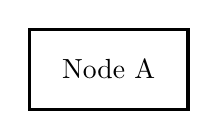
\begin{tikzpicture}
  \node[minimum width=2cm,minimum height=1cm] (A) {Node A};
  \tcbvignette{inside node=A}
  \draw[very thick] (A.south west) rectangle (A.north east);
\end{tikzpicture}
\end{dispExample*}
\end{vigTcbKey}

\clearpage

\begin{vigTcbKey}[][doc new=2016-04-22]{outside node}{=\meta{name}}{样式，初始 unset}
  将 \refCom{tcbvignette} 放置在给定 \meta{name} 的节点外部。
  \emph{装饰角}的内边界会适配该节点的几何尺寸。
\begin{dispExample*}{sbs,righthand width=3cm,center lower}
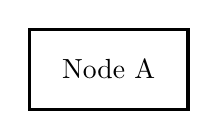
\begin{tikzpicture}
  \node[minimum width=2cm,minimum height=1cm] (A) {Node A};
  \tcbvignette{outside node=A}
  \draw[very thick] (A.south west) rectangle (A.north east);
\end{tikzpicture}
\end{dispExample*}
\end{vigTcbKey}


\begin{vigTcbKey}[][doc new=2016-04-22]{over node}{=\meta{name}}{样式，初始 unset}
  将 \refCom{tcbvignette} 叠加在给定 \meta{name} 的节点之上。
  \emph{装饰角}的外边界会适配该节点的几何尺寸，
  但会向外偏移 \refKey{/tcb/vig/over node offset}。
\begin{dispExample*}{sbs,righthand width=3cm,center lower}
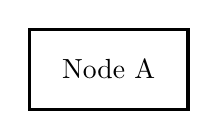
\begin{tikzpicture}
  \node[minimum width=2cm,minimum height=1cm] (A) {Node A};
  \tcbvignette{over node offset=1mm,over node=A}
  \draw[very thick] (A.south west) rectangle (A.north east);
\end{tikzpicture}
\end{dispExample*}
\end{vigTcbKey}

\begin{vigTcbKey}[][doc new=2016-04-22]{over node offset}{=\meta{length}}{无默认值，初始 |0.1mm|}
  设定 \refKey{/tcb/vig/over node} 的偏移量。
  注意：必须\emph{先}设置 \refKey{/tcb/vig/over node offset}，
  再使用 \refKey{/tcb/vig/over node}。
\end{vigTcbKey}


\begin{vigTcbKey}[][doc new=2016-04-22]{north size}{=\meta{length}}{无默认值，初始 |2mm|}
  设置北侧\emph{装饰角}部分的厚度。
\begin{dispExample*}{sbs,righthand width=3cm,center lower}
\begin{tikzpicture}
  \tcbvignette{north size=4mm}
\end{tikzpicture}
\end{dispExample*}
\end{vigTcbKey}

\begin{vigTcbKey}[][doc new=2016-04-22]{south size}{=\meta{length}}{无默认值，初始 |2mm|}
  设置南侧\emph{装饰角}部分的厚度。
\begin{dispExample*}{sbs,righthand width=3cm,center lower}
\begin{tikzpicture}
  \tcbvignette{south size=4mm}
\end{tikzpicture}
\end{dispExample*}
\end{vigTcbKey}

\begin{vigTcbKey}[][doc new=2016-04-22]{east size}{=\meta{length}}{无默认值，初始 |2mm|}
  设置东侧\emph{装饰角}部分的厚度。
\begin{dispExample*}{sbs,righthand width=3cm,center lower}
\begin{tikzpicture}
  \tcbvignette{east size=4mm}
\end{tikzpicture}
\end{dispExample*}
\end{vigTcbKey}

\begin{vigTcbKey}[][doc new=2016-04-22]{west size}{=\meta{length}}{无默认值，初始 |2mm|}
  设置西侧\emph{装饰角}部分的厚度。
\begin{dispExample*}{sbs,righthand width=3cm,center lower}
\begin{tikzpicture}
  \tcbvignette{west size=4mm}
\end{tikzpicture}
\end{dispExample*}
\end{vigTcbKey}

\clearpage

\begin{vigTcbKey}[][doc new=2016-04-22]{vertical size}{=\meta{length}}{样式，初始 |2mm|}
  将 \refKey{/tcb/vig/north size} 和 \refKey{/tcb/vig/south size}
  设置为给定的 \meta{length}。
\begin{dispExample*}{sbs,righthand width=3cm,center lower}
\begin{tikzpicture}
  \tcbvignette{vertical size=4mm}
\end{tikzpicture}
\end{dispExample*}
\end{vigTcbKey}

\begin{vigTcbKey}[][doc new=2016-04-22]{horizontal size}{=\meta{length}}{样式，初始 |2mm|}
  将 \refKey{/tcb/vig/east size} 和 \refKey{/tcb/vig/west size}
  设置为给定的 \meta{length}。
\begin{dispExample*}{sbs,righthand width=3cm,center lower}
\begin{tikzpicture}
  \tcbvignette{horizontal size=4mm}
\end{tikzpicture}
\end{dispExample*}
\end{vigTcbKey}


\begin{vigTcbKey}[][doc new=2016-04-22]{size}{=\meta{length}}{样式，初始 |2mm|}
  将 \refKey{/tcb/vig/north size}、\refKey{/tcb/vig/south size}、
  \refKey{/tcb/vig/east size} 和 \refKey{/tcb/vig/west size}
  都设置为给定的 \meta{length}。
\begin{dispExample*}{sbs,righthand width=3cm,center lower}
\begin{tikzpicture}
  \tcbvignette{size=4mm}
\end{tikzpicture}
\end{dispExample*}
\end{vigTcbKey}


\begin{marker}
\refKey{/tcb/vig/north size}、\refKey{/tcb/vig/south size} 等必须
在使用 \refKey{/tcb/vig/outside node} \emph{之前}设置。
\end{marker}



\subsection{通用颜色与样式设置}\label{subsec:vignettestyle}

\begin{vigTcbKey}[][doc new=2016-04-22]{north style}{=\marg{style}}{无默认值，初始 |red!50!white|}
  为北侧\emph{装饰角}部分设置 \tikzname\ \meta{style} 选项。
\begin{dispExample*}{sbs,righthand width=3cm,center lower}
\begin{tikzpicture}
  \tcbvignette{north style=blue}
\end{tikzpicture}
\end{dispExample*}
\end{vigTcbKey}

\begin{vigTcbKey}[][doc new=2016-04-22]{south style}{=\marg{style}}{无默认值，初始 |red!50!black|}
  为南侧\emph{装饰角}部分设置 \tikzname\ \meta{style} 选项。
\begin{dispExample*}{sbs,righthand width=3cm,center lower}
\begin{tikzpicture}
  \tcbvignette{south style={draw=blue,fill=yellow}}
\end{tikzpicture}
\end{dispExample*}
\end{vigTcbKey}


\begin{vigTcbKey}[][doc new=2016-04-22]{east style}{=\marg{style}}{无默认值，初始 |red!75!black|}
  为东侧\emph{装饰角}部分设置 \tikzname\ \meta{style} 选项。
\begin{dispExample*}{sbs,righthand width=3cm,center lower}
\begin{tikzpicture}
  \tcbvignette{east style={left color=yellow!75!black,
    right color=blue!75!black}}
\end{tikzpicture}
\end{dispExample*}
\end{vigTcbKey}

\clearpage

\begin{vigTcbKey}[][doc new=2016-04-22]{west style}{=\marg{style}}{无默认值，初始 |red!75!white|}
  为西侧\emph{装饰角}部分设置 \tikzname\ \meta{style} 选项。
\begin{dispExample*}{sbs,righthand width=3cm,center lower}
\begin{tikzpicture}
  \tcbvignette{west style={preaction={fill=black!20},
    pattern=checkerboard,
    pattern color=black!30}}
\end{tikzpicture}
\end{dispExample*}
\end{vigTcbKey}


\begin{vigTcbKey}[][doc new=2016-05-24]{scope}{=\marg{style}}{无默认值，初始为空}
  四个\emph{装饰角}部分在一个 \tikzname\ |scope| 环境内部绘制，
  该环境以给定的 \meta{style} 作为选项。
\begin{dispExample*}{sbs,righthand width=3cm,center lower}
\begin{tikzpicture}
  \tcbvignette{scope={transparency group,opacity=0.25}}
\end{tikzpicture}
\end{dispExample*}
\end{vigTcbKey}



\begin{vigTcbKey}[][doc new=2016-04-22]{raised color}{=\meta{color}}{无默认值}
  通过将以下四个样式选项
  \refKey{/tcb/vig/north style}、
  \refKey{/tcb/vig/south style}、
  \refKey{/tcb/vig/east style} 和
  \refKey{/tcb/vig/west style}
  设置为给定 \meta{color} 的加深与加亮变体，营造凸起的边框观感。
\begin{dispExample*}{sbs,righthand width=3cm,center lower}
\begin{tikzpicture}
  \tcbvignette{raised color=blue}
\end{tikzpicture}
\end{dispExample*}
\end{vigTcbKey}


\begin{vigTcbKey}[][doc new=2016-04-22]{lowered color}{=\meta{color}}{无默认值}
  通过将以下四个样式选项
  \refKey{/tcb/vig/north style}、
  \refKey{/tcb/vig/south style}、
  \refKey{/tcb/vig/east style} 和
  \refKey{/tcb/vig/west style}
  设置为给定 \meta{color} 的加深与加亮变体，营造凹陷的边框观感。
\begin{dispExample*}{sbs,righthand width=3cm,center lower}
\begin{tikzpicture}
  \tcbvignette{lowered color=green!75!black}
\end{tikzpicture}
\end{dispExample*}
\end{vigTcbKey}


\begin{vigTcbKey}[][doc new=2016-04-22]{color from}{=\meta{inner} |to| \meta{outer}}{无默认值}
  设置以下四个样式选项
  \refKey{/tcb/vig/north style}、
  \refKey{/tcb/vig/south style}、
  \refKey{/tcb/vig/east style} 和
  \refKey{/tcb/vig/west style}，
  使颜色从 \meta{inner} 色渐变到 \meta{outer} 色。
\begin{dispExample*}{sbs,righthand width=3cm,center lower}
\begin{tikzpicture}
  \tcbvignette{color from=red to blue!50}
\end{tikzpicture}
\end{dispExample*}
\end{vigTcbKey}



\begin{vigTcbKey}[][doc new=2016-04-22]{base color}{=\meta{color}}{无默认值}
  为 \refKey{/tcb/vig/raised color}、
  \refKey{/tcb/vig/lowered color}、\refKey{/tcb/finish fading vignette}
  设置基准颜色。通常无需直接设置此值。
\end{vigTcbKey}


\clearpage
\begin{vigTcbKey}[][doc new=2016-04-22]{draw method}{=\docValue{direct}\textbar\docValue{clipped}}{无默认值，初始 |direct|}
  尤其是在使用着色或褪色时，绘制出的\emph{装饰角}图形有时并不像预期那样完美。
  出现的瑕疵和缺陷很大程度上取决于预览软件。
  \refKey{/tcb/vig/draw method} 用于提供若干可选的替代绘制方法。
  \begin{itemize}
  \item\docValue{direct}：\emph{装饰角}各部分用单个 \tikzname\ 图形绘制/填充。
    对于实色图形，这是首选（也是默认）方法。
  \item\docValue{clipped}：\emph{装饰角}各部分绘制得略大一些，再裁剪到目标区域。
    配合着色和褪色使用时，这样似乎能得到更好/不同的视觉效果（取决于预览器）。
  \end{itemize}
\begin{dispExample*}{sbs,righthand width=3cm,center lower}
\begin{tikzpicture}
  \tcbvignette{color from=red to yellow}
\end{tikzpicture}
\end{dispExample*}
\begin{dispExample*}{sbs,righthand width=3cm,center lower}
\begin{tikzpicture}
  \tcbvignette{color from=red to yellow,draw method=clipped}
\end{tikzpicture}
\end{dispExample*}

\begin{marker}
本选项乃权宜之计，未来可能被修改或最好直接移除。
\end{marker}
\end{vigTcbKey}



\subsection{通用褪色设置}\label{subsec:vignettefading}

\tikzname\ 的 |fadings| 程序库 \cite{tantau:tikz_and_pgf}
由 \mylib{vignette} 程序库自动加载。
其中，|fadings| 程序库内部定义了
\docFading{west}、
\docFading{east}、
\docFading{north} 和
\docFading{south} 等褪色效果。

\mylib{vignette} 程序库又补充了若干褪色效果，即
\docFading{semi west}、
\docFading{semi east}、
\docFading{semi north} 和
\docFading{semi south}。
这些褪色效果比普通褪色效果\emph{弱}得多。

\begin{dispExample*}{sbs,righthand width=3cm,center lower}
\begin{tikzpicture}
  \fill [black!20] (0,0) rectangle (1,1);
  \path [pattern=checkerboard,pattern color=black!30]
    (0,0) rectangle (1,1);
  \fill [path fading=semi west,blue] (0,0) rectangle (1,1);
\end{tikzpicture}
\end{dispExample*}



\begin{tcboxedraster}{base example,title=褪色效果对比}
  \def\doShadingExample#1{%
    \begin{tcolorbox}[sbs,size=fbox,colback=white,lower separated=false,
      righthand width=2cm,left=5mm]
    \docFading{#1}\tcblower
    \begin{tikzpicture}
        \fill [black!20] (0,0) rectangle (1,1);
        \path [pattern=checkerboard,pattern color=black!30] (0,0) rectangle (1,1);
        \fill [path fading=#1,blue] (0,0) rectangle (1,1);
    \end{tikzpicture}
    \end{tcolorbox}}%
  \doShadingExample{west}
  \doShadingExample{east}
  \doShadingExample{north}
  \doShadingExample{south}
  \doShadingExample{semi west}
  \doShadingExample{semi east}
  \doShadingExample{semi north}
  \doShadingExample{semi south}
\end{tcboxedraster}


\clearpage

\begin{vigTcbKey}[][doc new=2016-04-22]{fade in}{\colOpt{=\marg{style}}}{样式，默认 |white|}
  设置以下四个样式选项
  \refKey{/tcb/vig/north style}、
  \refKey{/tcb/vig/south style}、
  \refKey{/tcb/vig/east style} 和
  \refKey{/tcb/vig/west style}，
  使路径从外向内褪色。
\begin{dispExample*}{sbs,righthand width=3cm,center lower}
\begin{tikzpicture}
  \fill [black!20] (-0.5,-0.5) rectangle (1.5,1.5);
  \path [pattern=checkerboard,pattern color=black!30]
    (-0.5,-0.5) rectangle (1.5,1.5);
  \tcbvignette{fade in=blue}
\end{tikzpicture}
\end{dispExample*}
\end{vigTcbKey}


\begin{vigTcbKey}[][doc new=2016-04-22]{fade out}{\colOpt{=\marg{style}}}{样式，默认 |white|}
  设置以下四个样式选项
  \refKey{/tcb/vig/north style}、
  \refKey{/tcb/vig/south style}、
  \refKey{/tcb/vig/east style} 和
  \refKey{/tcb/vig/west style}，
  使路径从内向外褪色。
\begin{dispExample*}{sbs,righthand width=3cm,center lower}
\begin{tikzpicture}
  \fill [black!20] (-0.5,-0.5) rectangle (1.5,1.5);
  \path [pattern=checkerboard,pattern color=black!30]
    (-0.5,-0.5) rectangle (1.5,1.5);
  \tcbvignette{fade out=blue}
\end{tikzpicture}
\end{dispExample*}
\end{vigTcbKey}


\begin{vigTcbKey}[][doc new=2016-04-22]{semi fade in}{\colOpt{=\marg{style}}}{样式，默认 |white|}
  设置以下四个样式选项
  \refKey{/tcb/vig/north style}、
  \refKey{/tcb/vig/south style}、
  \refKey{/tcb/vig/east style} 和
  \refKey{/tcb/vig/west style}，
  使路径从外向内弱褪色。
\begin{dispExample*}{sbs,righthand width=3cm,center lower}
\begin{tikzpicture}
  \fill [black!20] (-0.5,-0.5) rectangle (1.5,1.5);
  \path [pattern=checkerboard,pattern color=black!30]
    (-0.5,-0.5) rectangle (1.5,1.5);
  \tcbvignette{semi fade in=blue}
\end{tikzpicture}
\end{dispExample*}
\end{vigTcbKey}


\begin{vigTcbKey}[][doc new=2016-04-22]{semi fade out}{\colOpt{=\marg{style}}}{样式，默认 |white|}
  设置以下四个样式选项
  \refKey{/tcb/vig/north style}、
  \refKey{/tcb/vig/south style}、
  \refKey{/tcb/vig/east style} 和
  \refKey{/tcb/vig/west style}，
  使路径从内向外弱褪色。
\begin{dispExample*}{sbs,righthand width=3cm,center lower}
\begin{tikzpicture}
  \fill [black!20] (-0.5,-0.5) rectangle (1.5,1.5);
  \path [pattern=checkerboard,pattern color=black!30]
    (-0.5,-0.5) rectangle (1.5,1.5);
  \tcbvignette{semi fade out=blue}
\end{tikzpicture}
\end{dispExample*}
\end{vigTcbKey}

\clearpage

如有需要，还可以为装饰角的每一边分别指定不同的褪色效果。
为此，需借助以下四个样式选项逐一施加褪色效果：
  \refKey{/tcb/vig/north style}、
  \refKey{/tcb/vig/south style}、
  \refKey{/tcb/vig/east style} 和
  \refKey{/tcb/vig/west style}。
\begin{dispExample*}{sbs,righthand width=3cm,center lower}
\begin{tikzpicture}
  \fill [black!20] (-0.5,-0.5) rectangle (1.5,1.5);
  \path [pattern=checkerboard,pattern color=black!30]
    (-0.5,-0.5) rectangle (1.5,1.5);
  \tcbvignette{
    north style={blue,path fading=south},
    east style ={blue,path fading=semi west},
    south style={blue,path fading=semi north},
    west style ={blue,path fading=east}
  }
\end{tikzpicture}
\end{dispExample*}

\begin{dispExample*}{sbs,righthand width=3cm,center lower}
\begin{tikzpicture}
  \fill [black!20] (-0.5,-0.5) rectangle (1.5,1.5);
  \path [pattern=checkerboard,pattern color=black!30]
    (-0.5,-0.5) rectangle (1.5,1.5);
  \tcbvignette{
    north style={blue,path fading=west},
    east style ={blue,path fading=south},
    south style={red,path fading=east},
    west style ={red,path fading=north}
  }
\end{tikzpicture}
\end{dispExample*}


\clearpage
\subsection{作为底层的装饰角}\label{subsec:vignetteunderlay}

\begin{docTcbKey}[][doc new=2016-04-22]{underlay vignette}{\colOpt{=\marg{options}}}{样式，无默认值}
  这会将一个带有给定 \meta{options} 的 \refCom{tcbvignette}
  作为 \refKey{/tcb/underlay} 放置到 \refEnv{tcolorbox} 上。
  \emph{装饰角}的尺寸会与 \refEnv{tcolorbox} 的尺寸相匹配。
  例如，\refKey{/tcb/leftrule} 被用作 \refKey{/tcb/vig/west size}；
  \refKey{/tcb/colframe} 被用作 \refKey{/tcb/vig/raised color}。

  对于 \refKey{/tcb/breakable} 文本框，\emph{装饰角}也会随之断开。
  另一种做法是，配合适当的设置，直接在 \refKey{/tcb/underlay}
  中使用 \refCom{tcbvignette}。

\begin{dispExample*}{sbs,righthand width=3cm,center lower}
\begin{tcolorbox}[enhanced,size=small,sharp corners,
  colback=green!10,colframe=green!50!black,
  boxrule=2mm,titlerule=0mm,
  title=My title,center title,fonttitle=\bfseries,
  underlay vignette]
    This is a tcolorbox.
\end{tcolorbox}
\end{dispExample*}

\begin{dispExample*}{sbs,righthand width=3cm,center lower}
\begin{tcolorbox}[enhanced,size=small,arc=0pt,
  colback=blue!10,colframe=blue,boxrule=2mm,
  underlay vignette={size=1.5mm}]
    This is a tcolorbox.
\end{tcolorbox}
\end{dispExample*}

\begin{dispExample*}{sbs,righthand width=3cm,center lower}
\begin{tcolorbox}[enhanced,size=small,sharp corners,
  colframe=red,interior hidden,boxrule=2mm,
  colupper=white,center upper,fontupper=\bfseries,
  underlay vignette]
    This is a tcolorbox.
\end{tcolorbox}
\end{dispExample*}

\begin{dispExample*}{sbs,righthand width=3cm,center lower}
\begin{tcolorbox}[enhanced,size=small,sharp corners,
  colback=red!50!yellow,frame hidden,boxrule=2mm,
  underlay vignette={color from=red!50!yellow to white,
     draw method=clipped,size=2.1mm}]
    This is a tcolorbox.
\end{tcolorbox}
\end{dispExample*}

\begin{dispExample*}{sbs,righthand width=3cm,center lower}
\tcbox[enhanced,sharp corners,colback=red!10,colframe=red]
  {Test}

\tcbox[enhanced,sharp corners,colback=red!10,colframe=red,
  underlay vignette]{Test}
\end{dispExample*}

\end{docTcbKey}


\clearpage
\begin{docTcbKey}[][doc new=2016-04-22]{underlay raised shading vignette}{\colOpt{=\marg{options}}}{样式，无默认值}
  这是从 \refKey{/tcb/underlay vignette} 派生的一种特殊样式，
  它对边框颜色进行着色，营造柔和的凸起边框观感。

\begin{dispExample*}{sbs,righthand width=3cm,center lower}
\begin{tcolorbox}[enhanced,sharp corners,
  colback=green!10,
  colframe=green!50!black,
  size=small,boxrule=2mm,titlerule=0mm,
  title=My title,center title,fonttitle=\bfseries,
  underlay raised shading vignette]
    This is a tcolorbox.
\end{tcolorbox}
\end{dispExample*}
\end{docTcbKey}



\begin{docTcbKey}[][doc new=2016-04-22]{underlay raised fading vignette}{\colOpt{=\marg{options}}}{样式，无默认值}
  该样式产生与 \refKey{/tcb/underlay raised shading vignette} 类似的效果，
  但此处使用的是路径褪色。不同的视觉效果很大程度上取决于预览器。
\begin{dispExample*}{sbs,righthand width=3cm,center lower}
\begin{tcolorbox}[enhanced,sharp corners,
  colback=green!10,
  colframe=green!50!black,
  size=small,boxrule=2mm,titlerule=0mm,
  title=My title,center title,fonttitle=\bfseries,
  underlay raised fading vignette]
    This is a tcolorbox.
\end{tcolorbox}
\end{dispExample*}
\end{docTcbKey}

\begin{docTcbKey}[][doc new=2016-04-22]{underlay shade in vignette}{\colOpt{=\marg{options}}}{样式，无默认值}
  这是从 \refKey{/tcb/underlay vignette} 派生的一种特殊样式，
  它使边框颜色渐变融入内部颜色。
\begin{dispExample*}{sbs,righthand width=3cm,center lower}
\begin{tcolorbox}[enhanced,sharp corners,frame hidden,
  colback=green!10,
  colframe=green!50!black,
  size=small,boxrule=2mm,titlerule=0mm,
  underlay shade in vignette]
    This is a tcolorbox.
\end{tcolorbox}
\end{dispExample*}
\end{docTcbKey}


\clearpage
\subsection{作为收尾的装饰角}\label{subsec:vignettefinish}


\begin{docTcbKey}[][doc new=2016-04-22]{finish vignette}{\colOpt{=\marg{options}}}{样式，无默认值}
  这会将一个带有给定 \meta{options} 的 \refCom{tcbvignette}
  作为 \refKey{/tcb/finish} 放置到 \refEnv{tcolorbox} 上。
  默认样式通过以较低不透明度绘制黑白两色部分，营造凸起的边框观感。

\begin{dispExample*}{sbs,righthand width=3cm,center lower}
\begin{tcolorbox}[enhanced,size=small,
  colback=green!10,colframe=green!50!black,
  boxrule=0.5mm,titlerule=0mm,
  title=My title,center title,fonttitle=\bfseries,
  finish vignette={size=1mm}]
    This is a tcolorbox.
\end{tcolorbox}
\end{dispExample*}

\begin{dispExample*}{sbs,righthand width=3cm,center lower}
\tcbincludegraphics[blankest,width=3cm,
  finish vignette={size=3mm}]{pink_marble.png}
\end{dispExample*}
\end{docTcbKey}


\begin{docTcbKey}[][doc new=2016-04-22]{finish raised fading vignette}{\colOpt{=\marg{options}}}{样式，无默认值}
  这会将一个带有给定 \meta{options} 的 \refCom{tcbvignette}
  作为 \refKey{/tcb/finish} 放置到 \refEnv{tcolorbox} 上。
  默认样式通过绘制渐隐的黑白两色部分，营造柔和的凸起边框观感。

\begin{dispExample*}{sbs,righthand width=3cm,center lower}
\begin{tcolorbox}[enhanced,size=small,
  colback=green!10,colframe=green!50!black,
  boxrule=0.5mm,titlerule=0mm,
  title=My title,center title,fonttitle=\bfseries,
  finish raised fading vignette={size=1mm}]
    This is a tcolorbox.
\end{tcolorbox}
\end{dispExample*}

\begin{dispExample*}{sbs,righthand width=3cm,center lower}
\tcbincludegraphics[blankest,width=3cm,
  finish raised fading vignette={size=3mm}]{pink_marble.png}
\end{dispExample*}

\end{docTcbKey}


\clearpage
\begin{docTcbKey}[][doc new=2016-04-22]{finish fading vignette}{\colOpt{=\marg{options}}}{样式，无默认值}
  这会将一个带有给定 \meta{options} 的 \refCom{tcbvignette}
  作为 \refKey{/tcb/finish} 放置到 \refEnv{tcolorbox} 上。
  默认样式使文本框从内向外渐隐为白色。注意此处使用了
  \refKey{/tcb/vig/over node}。可调整 \refKey{/tcb/vig/over node offset}
  使其或多或少地覆盖文本框。褪色颜色可用
  \refKey{/tcb/vig/base color} 设置。

\begin{dispExample*}{sbs,righthand width=3cm,center lower}
\begin{tcolorbox}[enhanced,size=small,
  colback=green!10,colframe=green!50!black,
  boxrule=0.5mm,titlerule=0mm,
  title=My title,center title,fonttitle=\bfseries,
  finish fading vignette={size=2mm}]
    This is a tcolorbox.
\end{tcolorbox}
\end{dispExample*}

\begin{dispExample*}{sbs,righthand width=3cm,center lower}
\tcbincludegraphics[blankest,width=3cm,
  finish fading vignette={size=3mm}]{pink_marble.png}
\end{dispExample*}

\begin{dispExample*}{sbs,righthand width=3cm,center lower}
\begin{tcolorbox}[colback=blue!50!black,size=small,
  title=Example]
\tcbincludegraphics[blankest,
  finish fading vignette={base color=blue!50!black,size=3mm,
    over node offset=0.2mm}]{pink_marble.png}
\end{tcolorbox}
\end{dispExample*}

\end{docTcbKey}


\begin{dispExample*}{}
\begin{tcbitemize}[raster columns=3,bicolor,
  raster equal height,sharp corners,boxrule=2mm,
  colframe=red,colback=yellow!5,colbacklower=yellow!25!red!20]
\tcbitem A
\tcbitem[underlay vignette] B
\tcbitem[underlay={\tcbvignette{inside node=interior,
  lowered color=red,size=1mm}}] C
\tcbitem[underlay vignette,
  underlay={\tcbvignette{inside node=interior,
  lowered color=red,size=1mm}}] D
\tcbitem[boxrule=3mm,underlay vignette={size=2mm},
  underlay={\tcbvignette{inside node=interior,
  lowered color=red,size=1mm}}] E
\tcbitem[underlay raised shading vignette] F
\tcbitem[underlay raised shading vignette,
  underlay={\tcbvignette{inside node=interior,
  lowered color=red,size=1mm}}] G
\tcbitem[title=H1,underlay={\tcbvignette{inside node=interior,
  lowered color=red,size=1mm}},finish vignette] H2
\tcbitem[boxrule=0.25mm,colback=red!30,finish vignette] I1 \tcblower I2
\tcbitem[tile,colback=red!30,finish raised fading vignette] J1 \tcblower J2
\tcbitem[boxrule=1mm,underlay={\tcbvignette{inside node=interior,
  raised color=red,size=1mm}}] K
\tcbitem[boxrule=1mm,title=L1,underlay={\tcbvignette{inside node=title,
  lowered color=red,size=0.5mm}}] L2
\end{tcbitemize}
\end{dispExample*}
